\section{L'environnement de développement et choix techniques: }

\subsection{Introduction}
\noindent
Le développement de notre projet nécessite un ordinateur avec des spécifications puissantes pour plusieurs raisons telles que le développement de C\# dans Visual Studio, le lancement des containers Docker, le lancement et le stockage de données dans Elasticsearch, l'importation et l'utilisation de notre modèle Sentence-Transformers, et surtout l'exécution de la recherche vectorielle. C'est pour cette raison que nous disposons d'ordinateurs avec les spécifications mentionnées dans la section  de l'environnement matériel ci-dessous. \\
\citetitle{elastic:hardwarespecifications} (\cite{elastic:hardwarespecifications})

\subsection{L'environnement matériel}
\noindent
Dans la table~\ref{tab:compspec} nous mentionnons les spécifications des ordinateurs utilisés pour le développement de notre application: 

\begin{table}[H]
\centering
\begin{tabular}{|c|c|c|c|}
\hline
\rowcolor{blue!20}
\textbf{Processeur} & \textbf{Mémoire} & \textbf{Disque dur} & \textbf{Système d'exploitation} \\
\hline
11th Gen Intel Core i7 @ 2.304GHz & 32Go & 1.5To SSD & Windows 11-64bits \\
\hline
9th Gen Intel Core i7 @ 1.8GHz & 32Go & 1To SSD 1To HDD & Windows 10-64bits \\
\hline
\end{tabular}
\caption{Spécifications des ordinateurs utilisés}
\label{tab:compspec}
\end{table}

\newpage
\subsection{L'environnement logiciel}
\noindent
{\small\textbf{\textit{Visual Studio}}}\mbox{}\\
Visual Studio est un environnement de développement intégré (IDE) créé par Microsoft. Il est principalement utilisé pour le développement de logiciels, notamment pour les langages de programmation tels que C\#, C++. Pour C\# il offre beacoup d'outils qui aident et accélérent et améliorent l'expérience de développement comme une complétion automatique intelligente, création des classes/interfaces intelligente et un débogeur puissant pour détecter et résoudre les erreurs. La figure ~\ref{fig:vs} présente le logo de Visual Studio.

\begin{figure}[H]
\centering

\includegraphics[width=0.3\textwidth]{logos/vs.png}
\caption{Logo officiel du logiciel Visual Studio}
\label{fig:vs}
\end{figure}

\noindent
{\small\textbf{\textit{Visual Studio Code}}}\mbox{}\\
Visual Studio Code (VS Code) est un éditeur du code source gratuit et open source développé par Microsoft connu par sa légéretè, rapidité et personnalisation à travers les extensions qu'il fournit pour une diversité des langages de programmation.
Il fournit beaucoup de choses qu'un IDE fait comme la coloration syntaxique, la complétion automatique, le déboggage, et la gestion de versions intégré. La figure ~\ref{fig:vsc} présente le logo de Visual Studio Code.
\begin{figure}[H]
\centering

\includegraphics[width=0.3\textwidth]{logos/vsc.png}
\caption{Logo officiel du logiciel Visual Studio Code}
\label{fig:vsc}
\end{figure}

\noindent
{\small\textbf{\textit{C\#}}}\mbox{}\\
C\# (prononcé "C sharp") est un langage de programmation de haut niveau, orienté objet, développé par Microsoft dans le cadre de sa plateforme .NET. Lancé en 2000, C\# a été conçu pour être simple, moderne, sûr et évolutif. C\# est utilisé pour le développement  d'une variété d'applications, nottament des applications backend et des REST API web avec ASP .NET Core. La figure ~\ref{fig:cs} présente le logo de C\#.
\begin{figure}[H]
\centering

\includegraphics[width=0.3\textwidth]{logos/csharp.png}
\caption{Logo officiel du langage de programmation C\#}
\label{fig:cs}
\end{figure}

\noindent
{\small\textbf{\textit{ASP .NET Core}}}\mbox{}\\
ASP.NET Core est un framework open source développé par Microsoft pour la création d'applications web modernes. Il constitue la prochaine évolution de la plateforme ASP.NET, offrant une architecture modulaire, légère et hautement performante. Il offre une large flexibilité et une modularité au développeurs, il prend en charge principalement le développement des APIs web RESTful qui peuvent être déployé sur Windows, Linux et MacOS. Il offre une variété de fonctionallités comme le traitement asynchrone des requêtes, le middleware et le pipeline de requêtes personnalisable.
la figure ~\ref{fig:netcore} présente le logo de ASP .NET Core.
\begin{figure}[H]
\centering

\includegraphics[width=0.3\textwidth]{logos/dotnetcore.png}
\caption{Logo officiel du framework ASP .NET Core}
\label{fig:netcore}
\end{figure}

\noindent
{\small\textbf{\textit{Python}}}\mbox{}\\
Python est un langage de programmation interprété, de haut niveau, polyvalent puisqu'il est utilisé dans plusieurs domaines notamment l'analyse de données et le machine learning (avec des bibliothèques telles que NumPy, Pandas, et PyTorch). La figure ~\ref{fig:py} présente le logo de Python.
\begin{figure}[H]
\centering

\includegraphics[width=0.3\textwidth]{logos/pypng.png}
\caption{Logo officiel du langage de programmation Python}
\label{fig:py}
\end{figure}

\noindent
{\small\textbf{\textit{Jupyter Notebook}}}\mbox{}\\
Jupyter Notebook est une application web open source qui permet de créer et de partager des documents interactifs contenant du code qui sont composés des cellules de code qui peuvent être exécuté individuellement, et facilement partagé à travers de differents sites comme Kaggle, Google Collab. La figure ~\ref{fig:jupyter} présente le logo de Jupyter.
\begin{figure}[H]
\centering

\includegraphics[width=0.3\textwidth]{logos/jupyter.png}
\caption{Logo officiel du framework Jupyter}
\label{fig:jupyter}
\end{figure}


\noindent
{\small\textbf{\textit{Flask}}}\mbox{}\\
Flask est un framework Python trés minimalistique pour développer des REST APIs en Python. Il est très facile de configurer et de faire fonctionner une API. Et pour cette raison, nous l'avons utilisé pour exposer un point de terminaison d'API REST unique afin d'exposer notre modèle Sentence-Transformers. La figure ~\ref{fig:flask} présente le logo de Flask.
\begin{figure}[H]
\centering

\includegraphics[width=0.3\textwidth]{logos/flask.png}
\caption{Logo officiel du framework Flask}
\label{fig:flask}
\end{figure}


\noindent
{\small\textbf{\textit{React}}}\mbox{}\\
React est un framework Javascript gratuit et open-source développé et maintenu par méta(anciennement sous le nom Facebook) en 2013 utilisé principalement pour le développement des interfaces utilisateurs web complexes à travers des "components", ou composants en français. La figure ~\ref{fig:react} présente le logo de React.
\begin{figure}[H]
\centering

\includegraphics[width=0.3\textwidth]{logos/react.png}
\caption{Logo officiel de bibilothèque React}
\label{fig:react}
\end{figure}

\noindent
{\small\textbf{\textit{Typescript}}}\mbox{}\\
Typescript est un langage de programmation gratuit et open-source développé et maintenu par Microsoft principalement pour améliorer l'expérience de développement pour les développeurs Javascript en fournissant des types statiques, des erreurs directement dans l'éditeur de code, et support total pour la programmation Orientée Objet. La figure ~\ref{fig:typescript} présente le logo de Typescript.
\begin{figure}[H]
\centering

\includegraphics[width=0.3\textwidth]{logos/typescript.png}
\caption{Logo officiel du langage Typescript}
\label{fig:typescript}
\end{figure}

\noindent
{\small\textbf{\textit{Docker}}}\mbox{}\\
Docker est une plateforme open source qui permet de développer, déployer et exécuter des applications de manière efficace en utilisant des conteneurs logiciels. Les conteneurs sont des unités d'exécution légères et autonomes qui encapsulent une application et tous ses composants, y compris les bibliothèques, la version de langages de programmation utilisèe(s), les ports exposés... 
la figure ~\ref{fig:docker} présente le logo de Docker.
\begin{figure}[H]
\centering

\includegraphics[width=0.3\textwidth]{logos/docker.png}
\caption{Logo officiel du Docker}
\label{fig:docker}
\end{figure}

\noindent
{\small\textbf{\textit{Elasticsearch}}}\mbox{}\\
Elasticsearch est un outil d'analyse de données distribuées open source et hautement èvolutif. Il est conçu pour stocker, rechercher et analyser et rechercher de grandes volumes de données de manière rapide et efficace en utilisant de diffèrentes mèthodes comme Knn Search.
Il utilise une structure de données de type index inversé pour indexer et rechercher rapidement des documents. Il prend en charge une variété de types de données, notamment le texte, les nombres, les dates, et les vecteurs par exemple le type dense vector.
La figure ~\ref{fig:elasticsearch} présente le logo d'Elasticsearch.
\begin{figure}[H]
\centering

\includegraphics[width=0.3\textwidth]{logos/elasticsearch.png}
\caption{Logo officiel d'Elasticsearch}
\label{fig:elasticsearch}
\end{figure}

\noindent
{\small\textbf{\textit{Kibana}}}\mbox{}\\
Kibana est un logiciel de visualisation de données liées à Elasticsearch. Il permet de visualiser et manipuler les indexes stockées dans Elasticsearch ainsi que l'analyse des données de grandes volumes.
La figure ~\ref{fig:kibana} présente le logo de Kibana.
\begin{figure}[H]
\centering

\includegraphics[width=0.3\textwidth]{logos/kibana.png}
\caption{Logo officiel du Kibana}
\label{fig:kibana}
\end{figure}

\noindent
{\small\textbf{\textit{Postman}}}\mbox{}\\
Postman est une plateforme API qui permet de construire, tester et utiliser des APIs en simplifiant et organisant les étapes nécessaires comme la création des workspaces, qui permet au utilisateurs de regrouper plusieurs endpoints API dans un workspace aussi que le support de différents types de "body". La figure ~\ref{fig:postman} présente le logo de Postman
\begin{figure}[H]
\centering

\includegraphics[width=0.3\textwidth]{logos/postman.png}
\caption{Logo officiel du logiciel Postman}
\label{fig:postman}
\end{figure}

\noindent
{\small\textbf{\textit{Overleaf}}}\mbox{}\\
Overleaf est une plateforme en ligne permettant un éditeur de texte pour LaTeX sans aucun téléchargement de logiciel, aussi connu comme un SaaS (Software as a Service). Il permet l'écriture collaborative des documents comme celui-ci.
La figure ~\ref{fig:overleaf} présente le logo d'Overleaf.
\begin{figure}[H]
\centering

\includegraphics[width=0.3\textwidth]{logos/overleaf.png}
\caption{Logo officiel du Overleaf}
\label{fig:overleaf}
\end{figure}

\noindent
{\small\textbf{\textit{LaTeX}}}\mbox{}\\
LaTeX utilise des commandes de texte pour indiquer comment le document doit être structuré et formaté, plutôt que se concentrer sur la présentation visuelle. Le document est ensuite compilé en un fichier de format PDF en appliquant les régles typographiques et la mise en page appuyée. La figure ~\ref{fig:latex} présente le logo de LaTeX
\begin{figure}[H]
\centering

\includegraphics[width=0.3\textwidth]{logos/latex.png}
\caption{Logo officiel du LaTeX}
\label{fig:latex}
\end{figure}

\subsection{Logiciel de modélisation UML}
\noindent
{\small\textbf{\textit{Visual Paradigm}}}\mbox{}\\
Visual Paradigm est un outil de conception de diagrammes UML.Il est capable de prendre en charge de nombreux diagrammes commer-ciaux et techniques comme UML et BPMN. Cette plateforme possède une interface graphique simplifiant la manipulation de ces fonctionallités comme (Drag \& Drop). La figure ~\ref{fig:vp} présente le logo de Visual Paradigm.

\begin{figure}[H]
\centering

\includegraphics[width=0.3\textwidth]{logos/vp.png}
\caption{Logo officiel du Visual Paradigm}
\label{fig:vp}
\end{figure}

\newpage
\section{Diagramme de déploiement}
\noindent
Un diagramme de déploiement est une représentation visuelle de la configuration
matérielle et logicielle d'une application, ainsi que des connexions entre les différents composants. Il permet de comprendre comment les différents éléments de l'application sont déployés et interagissent les uns avec les autres. La figure ~\ref{fig:diagdepglobal} présente le diagramme de déploiement de notre application. On peut observer que notre serveur d'application est connecté a un serveur web Kestrel de .NET, aussi que deux bases de données, Elasticsearch, et MySQL, et qu'on a deux services API, ASP .NET Core et Flask qui contient notre modèle Sentence-Transformers.


\begin{figure}[H]
\centering
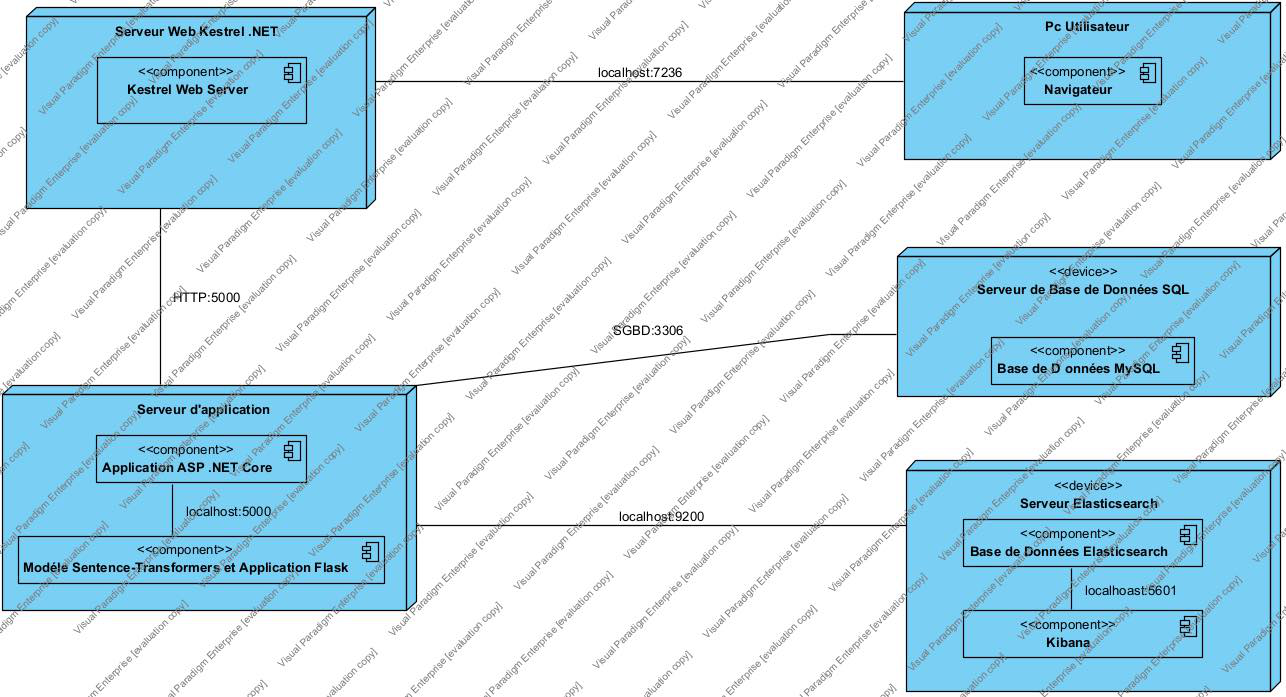
\includegraphics[width=1\textwidth]{logos/deployment.png}
\caption{Présentation du Diagramme de déploiement global}
\label{fig:diagdepglobal}
\end{figure}


\section{Conclusion}
\noindent
Dans ce chapitre, nous avons préparé notre plan de travail. Nous avons capturé les besoins fonctionnels et non fonctionnels de notre applcation et nous avons fixé nos choix techniques .
Dans le chapitre qui suit nous allons présenter le premier sprint. 